% auto-generated by tools/make_figures_tex.py
\begin{figure}[htbp]\centering
\begin{subfigure}{0.48\textwidth}\centering
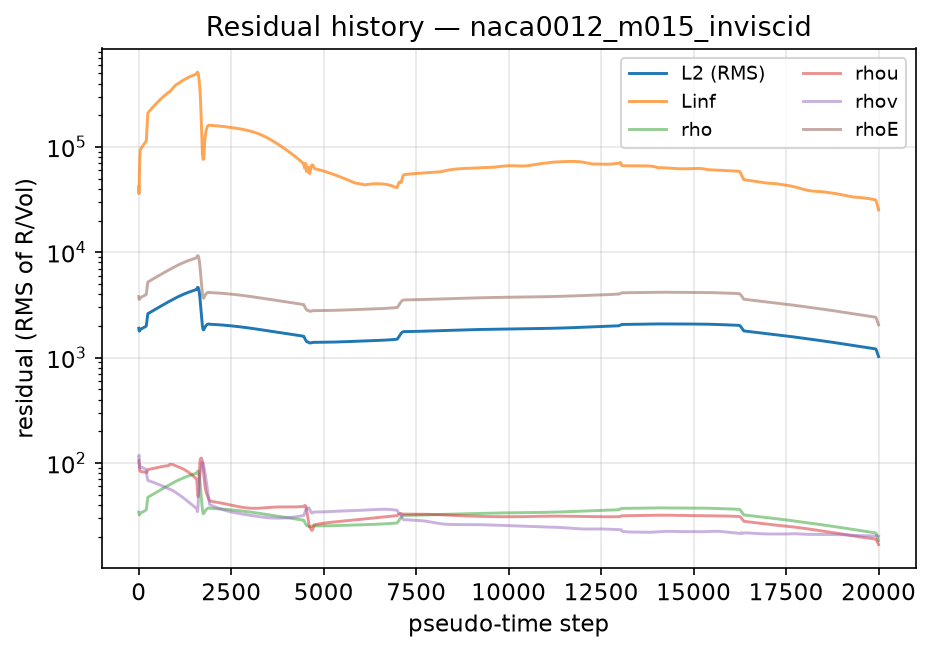
\includegraphics[width=\textwidth]{figures/naca0012_m015_inviscid_residuals.png}
\caption{residual history}
\end{subfigure}\hfill
\begin{subfigure}{0.48\textwidth}\centering
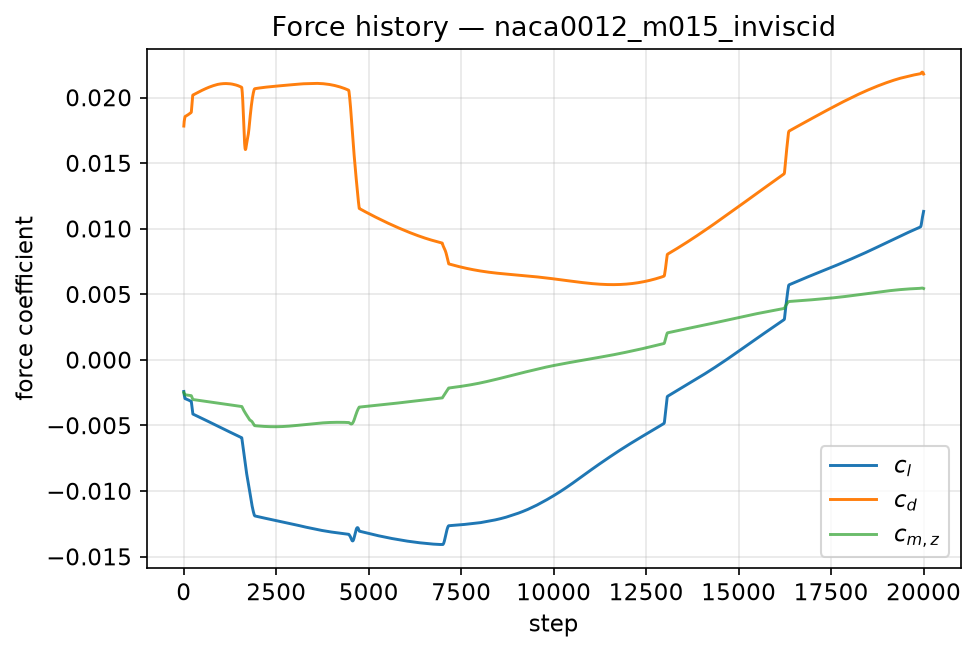
\includegraphics[width=\textwidth]{figures/naca0012_m015_inviscid_forces.png}
\caption{force history}
\end{subfigure}\hfill

\begin{subfigure}{0.48\textwidth}\centering
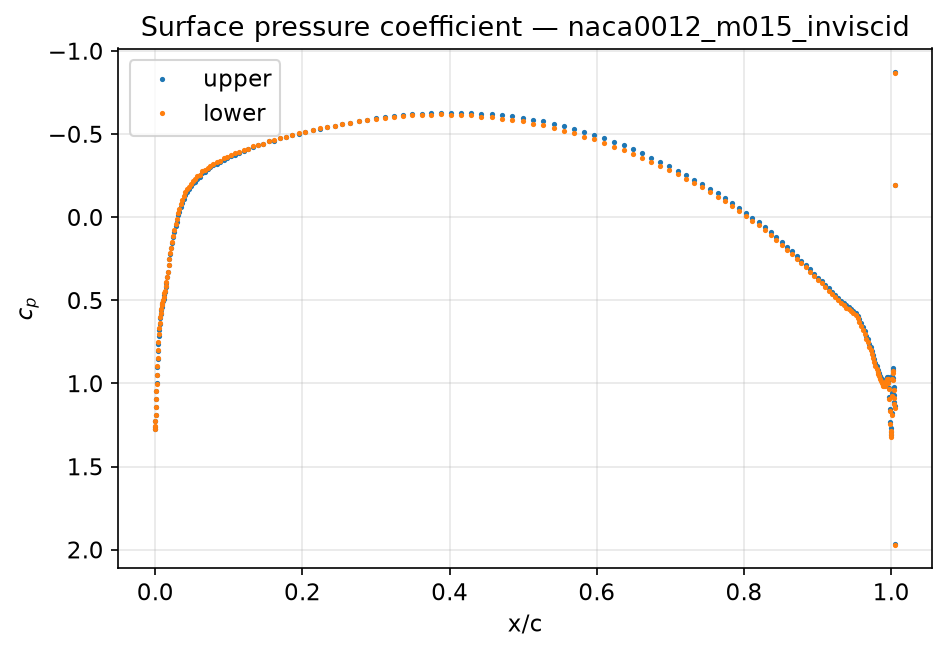
\includegraphics[width=\textwidth]{figures/naca0012_m015_inviscid_surface_cp.png}
\caption{surface $c_p$}
\end{subfigure}\hfill
\begin{subfigure}{0.48\textwidth}\centering
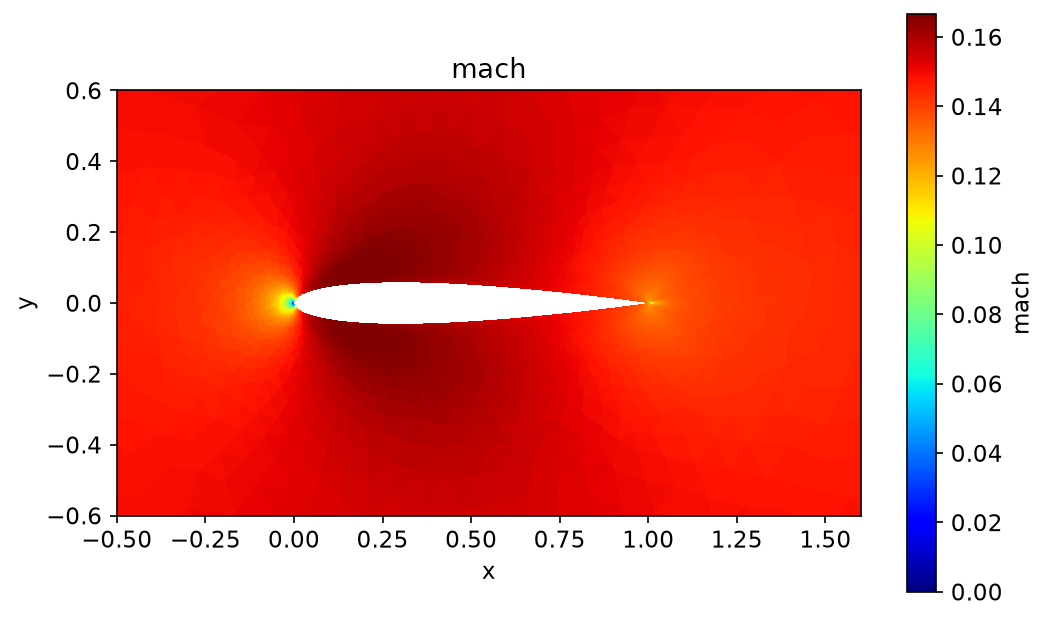
\includegraphics[width=\textwidth]{figures/naca0012_m015_inviscid_mach_zoom.png}
\caption{Mach (near body)}
\end{subfigure}\hfill

\begin{subfigure}{0.48\textwidth}\centering
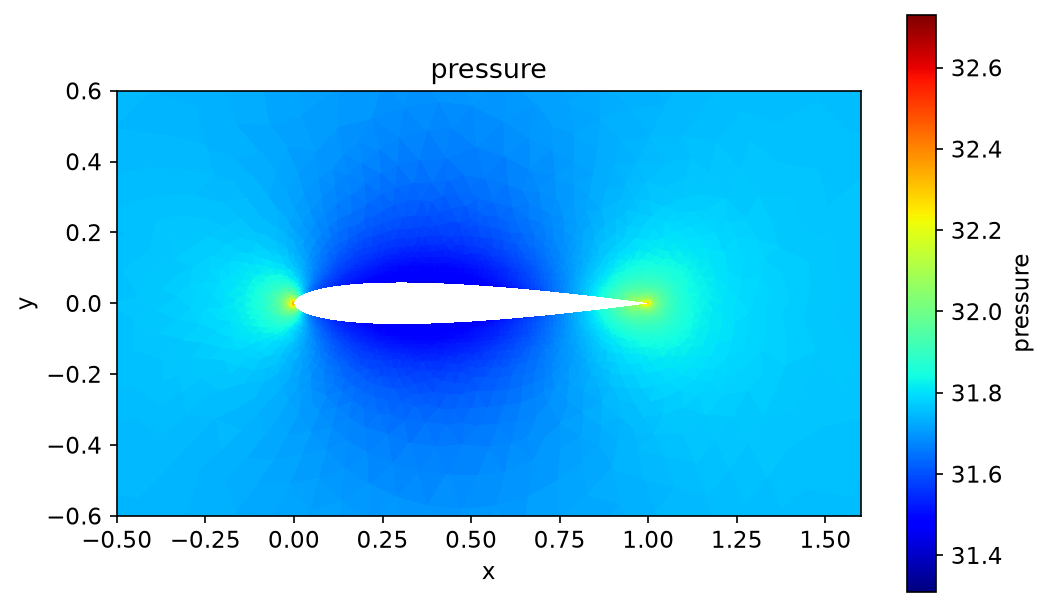
\includegraphics[width=\textwidth]{figures/naca0012_m015_inviscid_pressure_zoom.png}
\caption{pressure (near body)}
\end{subfigure}\hfill
\caption{Case \texttt{naca0012\_m015\_inviscid}: residual and force histories, surface distributions, and field contours. Plotted variables are named in each subcaption.}
\label{fig:m015inv}
\end{figure}

\begin{figure}[htbp]\centering
\begin{subfigure}{0.48\textwidth}\centering
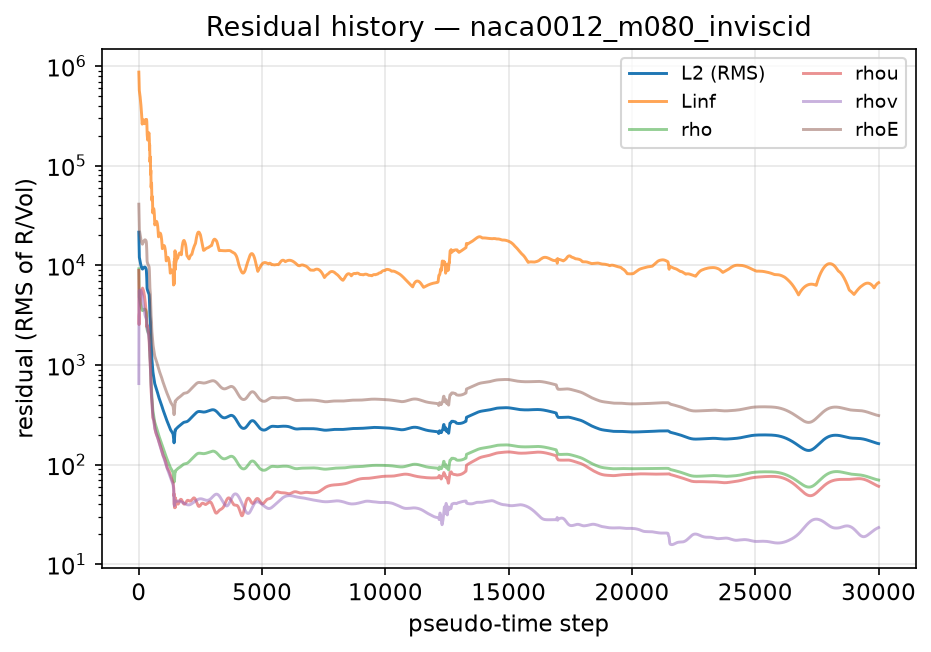
\includegraphics[width=\textwidth]{figures/naca0012_m080_inviscid_residuals.png}
\caption{residual history}
\end{subfigure}\hfill
\begin{subfigure}{0.48\textwidth}\centering
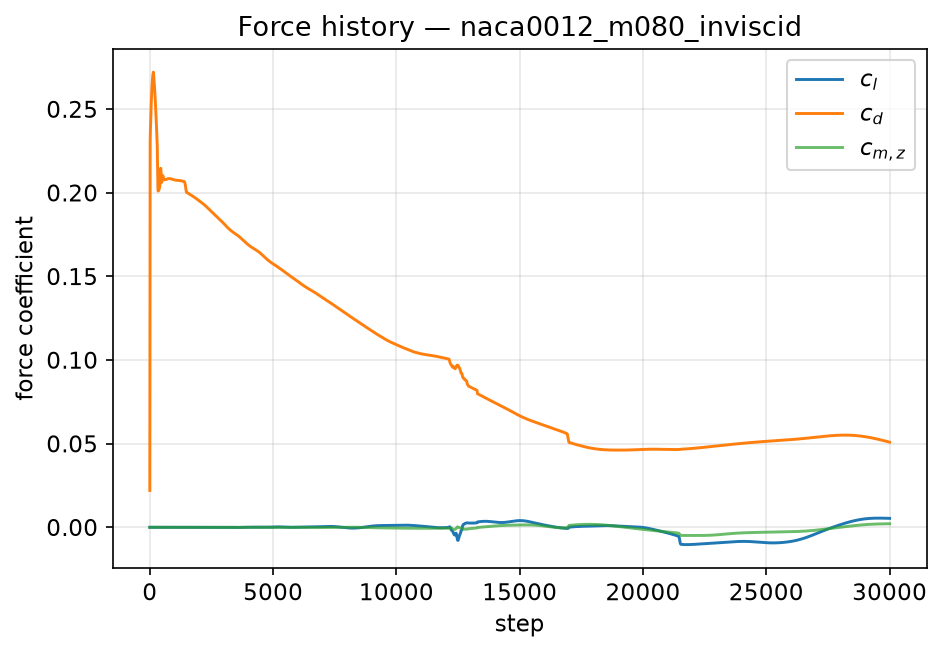
\includegraphics[width=\textwidth]{figures/naca0012_m080_inviscid_forces.png}
\caption{force history}
\end{subfigure}\hfill

\begin{subfigure}{0.48\textwidth}\centering
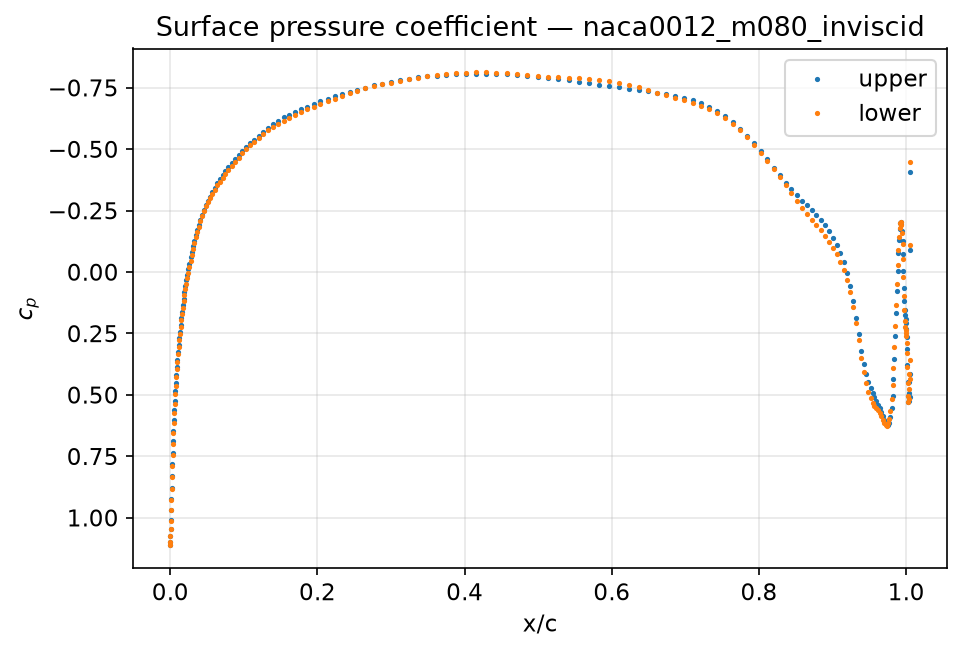
\includegraphics[width=\textwidth]{figures/naca0012_m080_inviscid_surface_cp.png}
\caption{surface $c_p$}
\end{subfigure}\hfill
\begin{subfigure}{0.48\textwidth}\centering
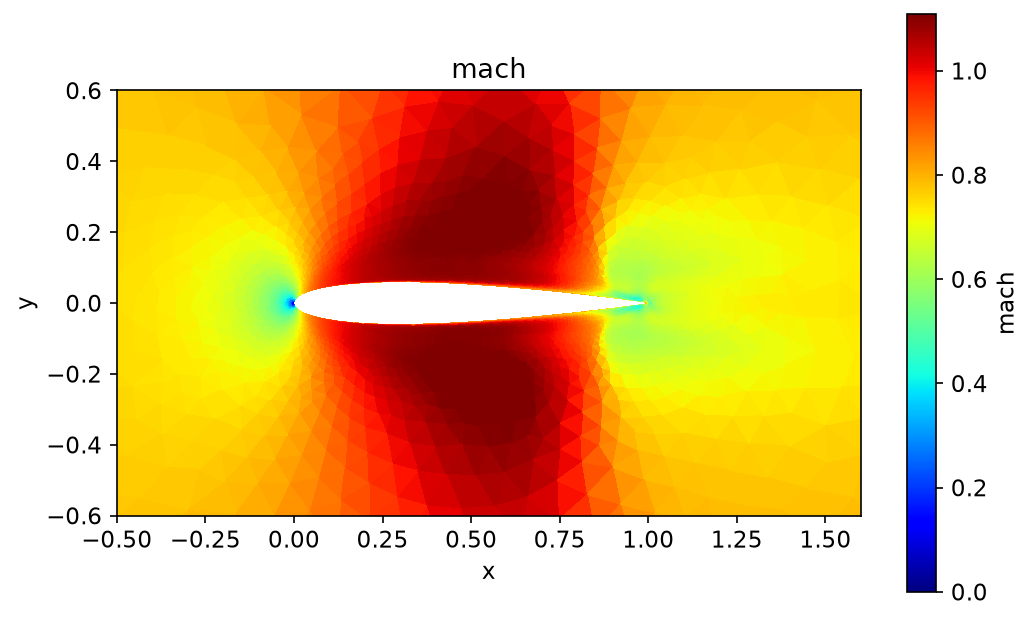
\includegraphics[width=\textwidth]{figures/naca0012_m080_inviscid_mach_zoom.png}
\caption{Mach (near body)}
\end{subfigure}\hfill

\begin{subfigure}{0.48\textwidth}\centering
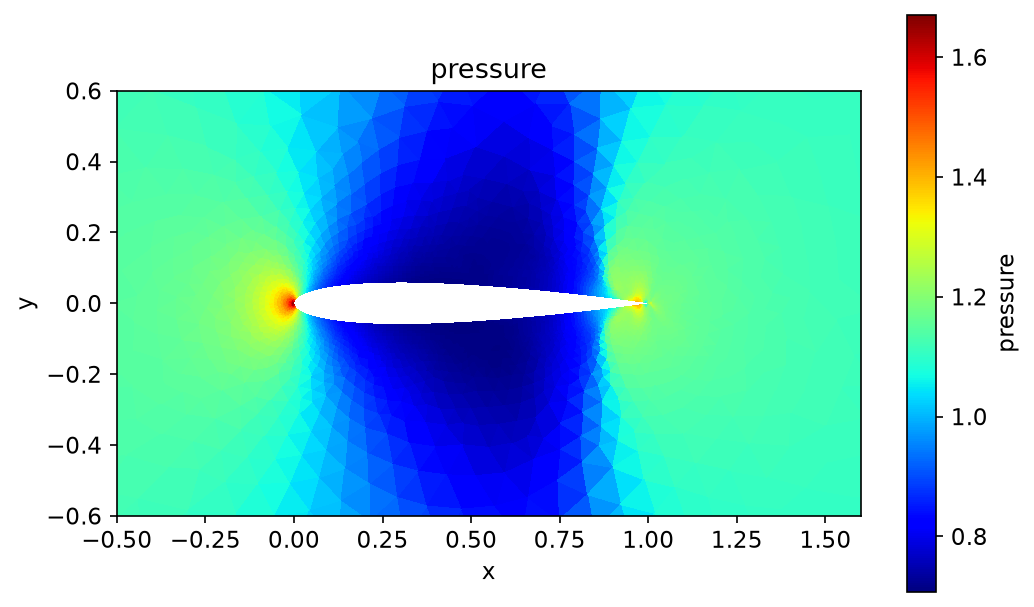
\includegraphics[width=\textwidth]{figures/naca0012_m080_inviscid_pressure_zoom.png}
\caption{pressure (near body)}
\end{subfigure}\hfill
\caption{Case \texttt{naca0012\_m080\_inviscid}: residual and force histories, surface distributions, and field contours. Plotted variables are named in each subcaption.}
\label{fig:m080inv}
\end{figure}

\begin{figure}[htbp]\centering
\begin{subfigure}{0.48\textwidth}\centering
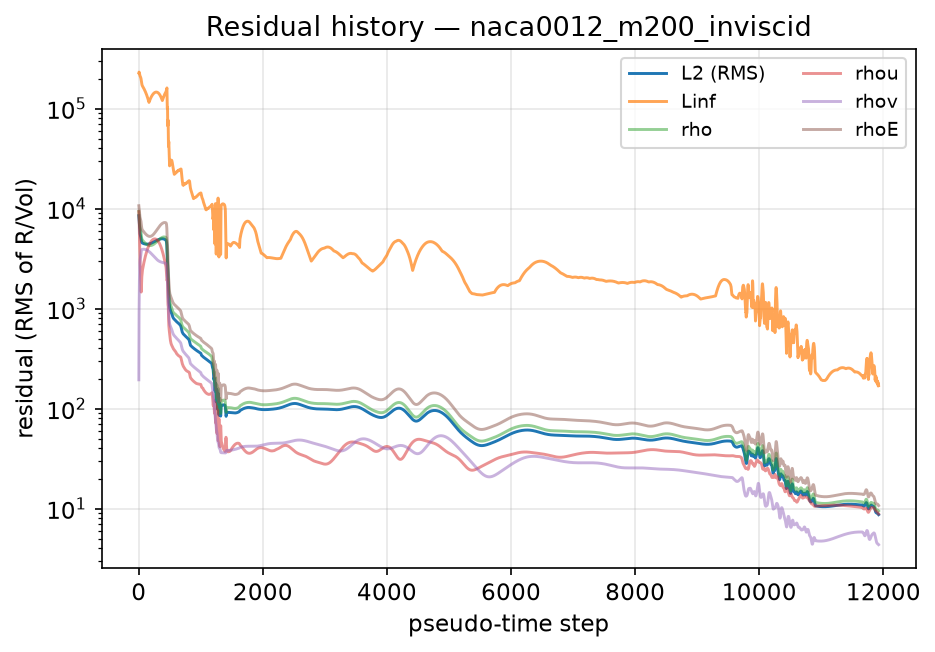
\includegraphics[width=\textwidth]{figures/naca0012_m200_inviscid_residuals.png}
\caption{residual history}
\end{subfigure}\hfill
\begin{subfigure}{0.48\textwidth}\centering
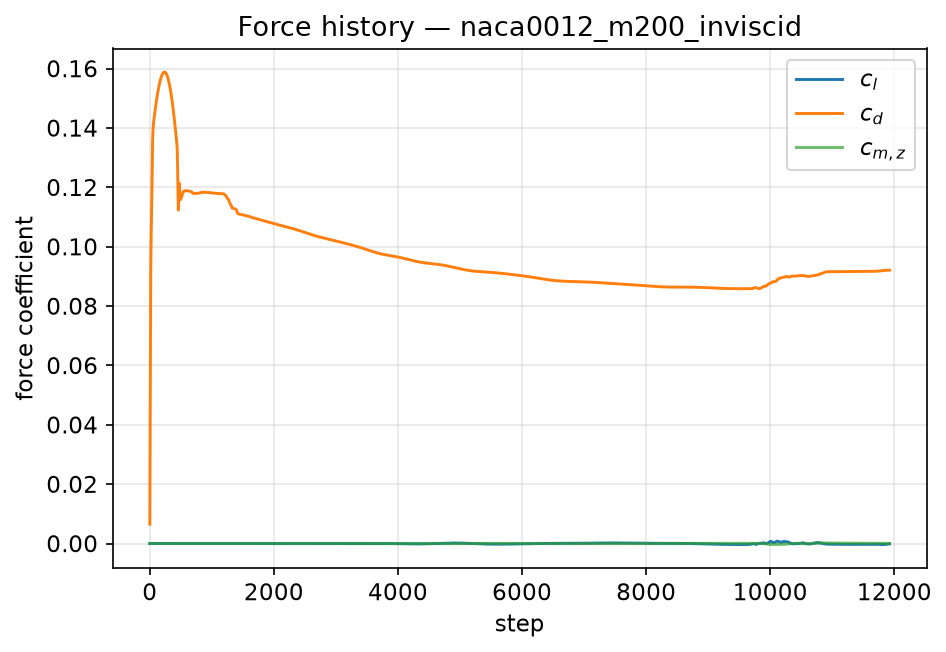
\includegraphics[width=\textwidth]{figures/naca0012_m200_inviscid_forces.png}
\caption{force history}
\end{subfigure}\hfill

\begin{subfigure}{0.48\textwidth}\centering
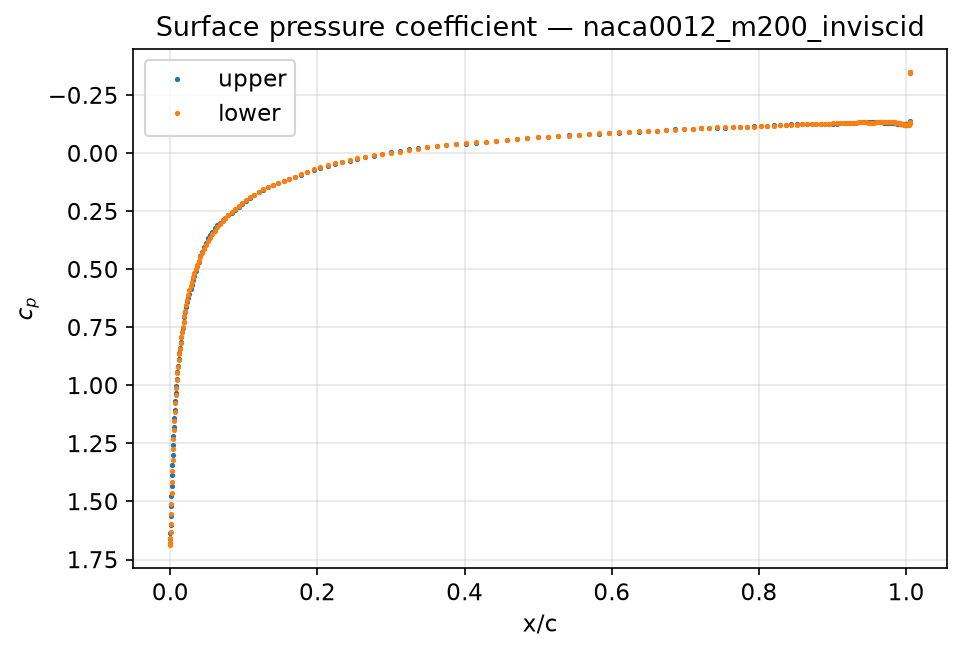
\includegraphics[width=\textwidth]{figures/naca0012_m200_inviscid_surface_cp.png}
\caption{surface $c_p$}
\end{subfigure}\hfill
\begin{subfigure}{0.48\textwidth}\centering
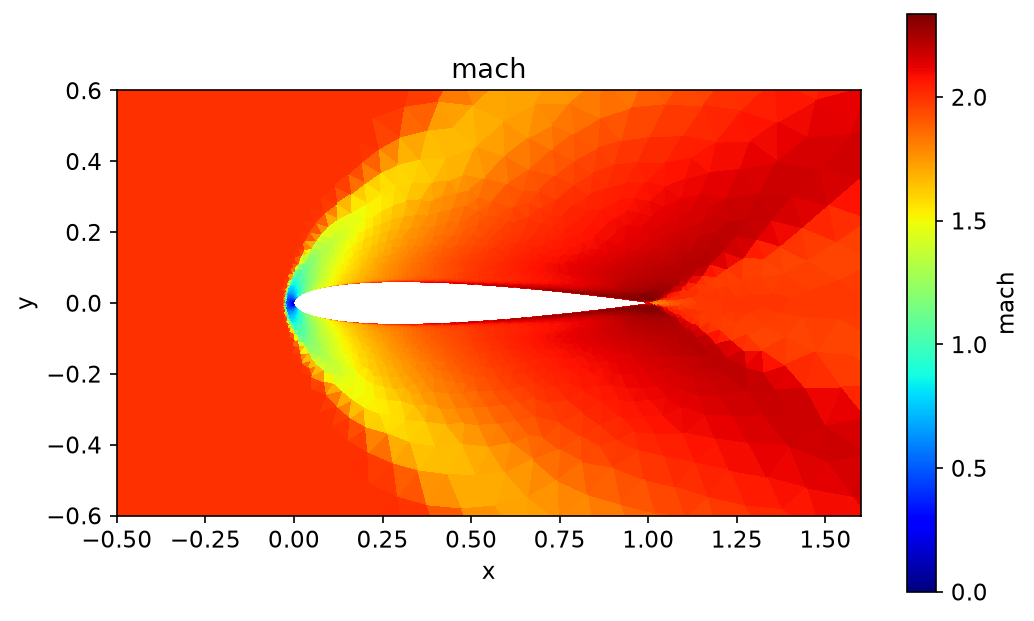
\includegraphics[width=\textwidth]{figures/naca0012_m200_inviscid_mach_zoom.png}
\caption{Mach (near body)}
\end{subfigure}\hfill

\begin{subfigure}{0.48\textwidth}\centering
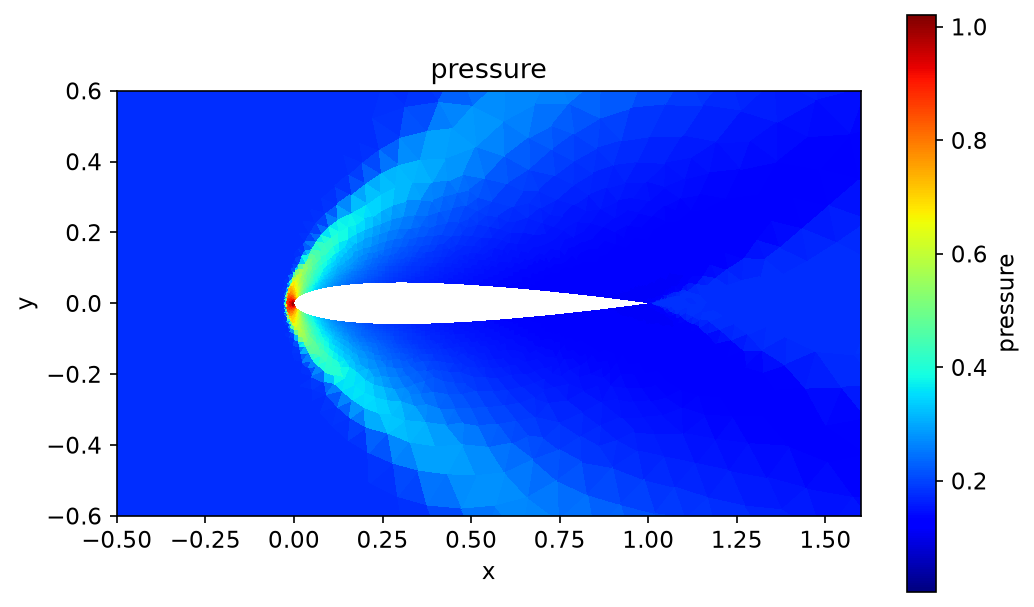
\includegraphics[width=\textwidth]{figures/naca0012_m200_inviscid_pressure_zoom.png}
\caption{pressure (near body)}
\end{subfigure}\hfill
\caption{Case \texttt{naca0012\_m200\_inviscid}: residual and force histories, surface distributions, and field contours. Plotted variables are named in each subcaption.}
\label{fig:m200inv}
\end{figure}

\begin{figure}[htbp]\centering
\begin{subfigure}{0.48\textwidth}\centering
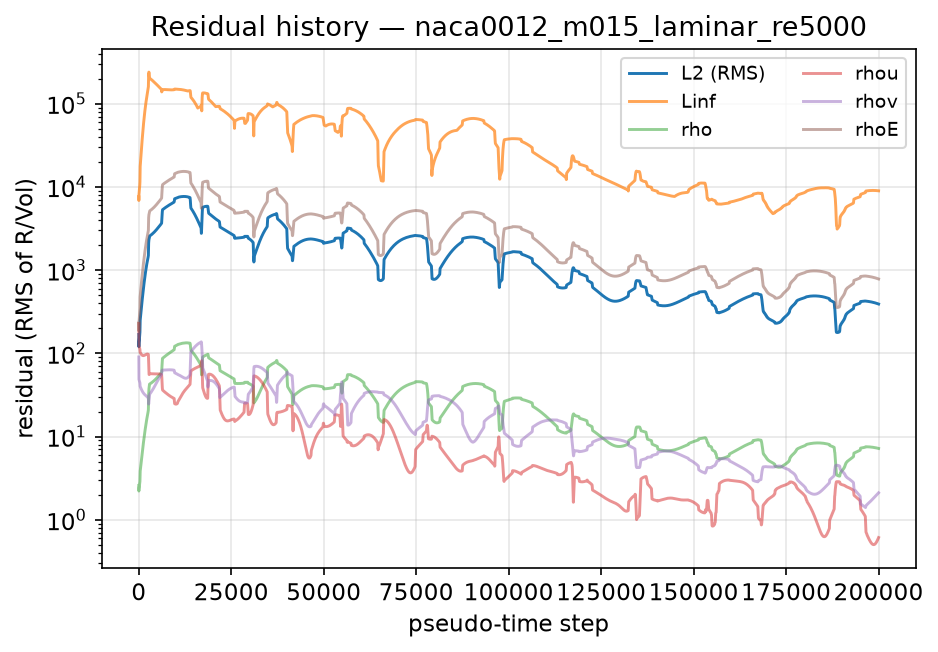
\includegraphics[width=\textwidth]{figures/naca0012_m015_laminar_re5000_residuals.png}
\caption{residual history}
\end{subfigure}\hfill
\begin{subfigure}{0.48\textwidth}\centering
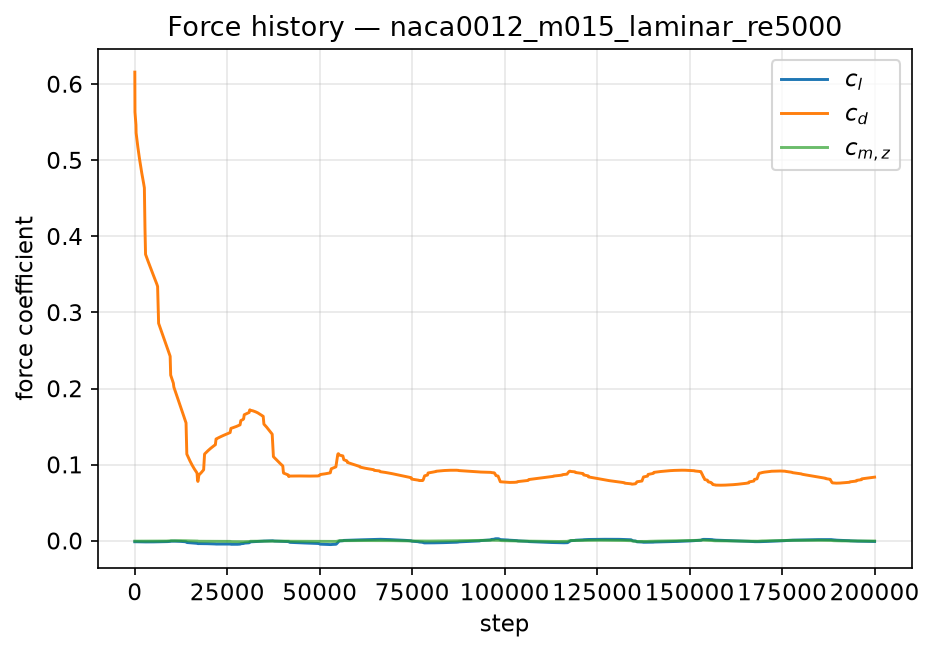
\includegraphics[width=\textwidth]{figures/naca0012_m015_laminar_re5000_forces.png}
\caption{force history}
\end{subfigure}\hfill

\begin{subfigure}{0.48\textwidth}\centering
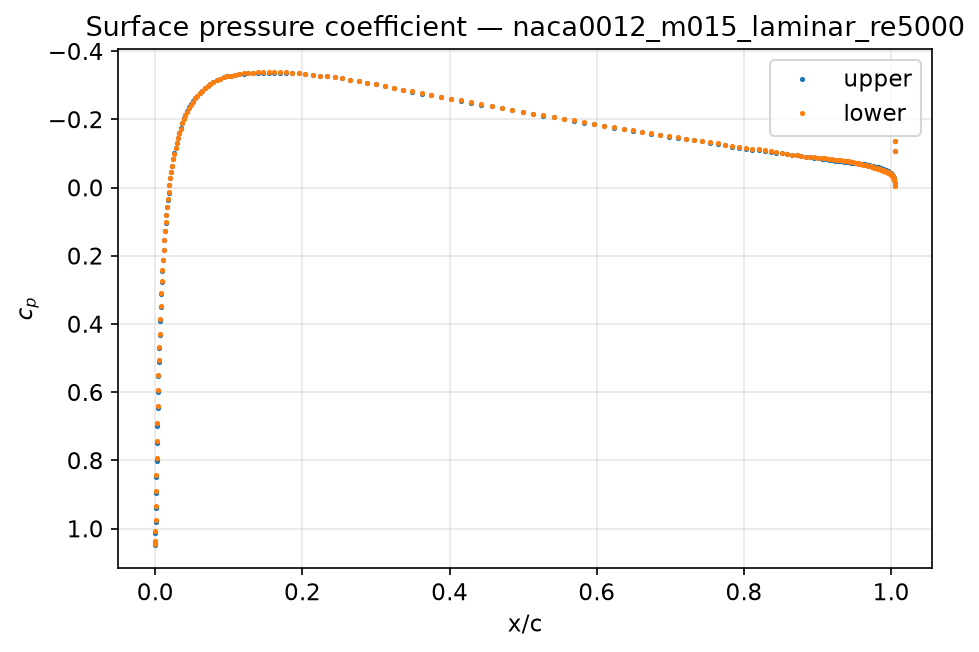
\includegraphics[width=\textwidth]{figures/naca0012_m015_laminar_re5000_surface_cp.png}
\caption{surface $c_p$}
\end{subfigure}\hfill
\begin{subfigure}{0.48\textwidth}\centering
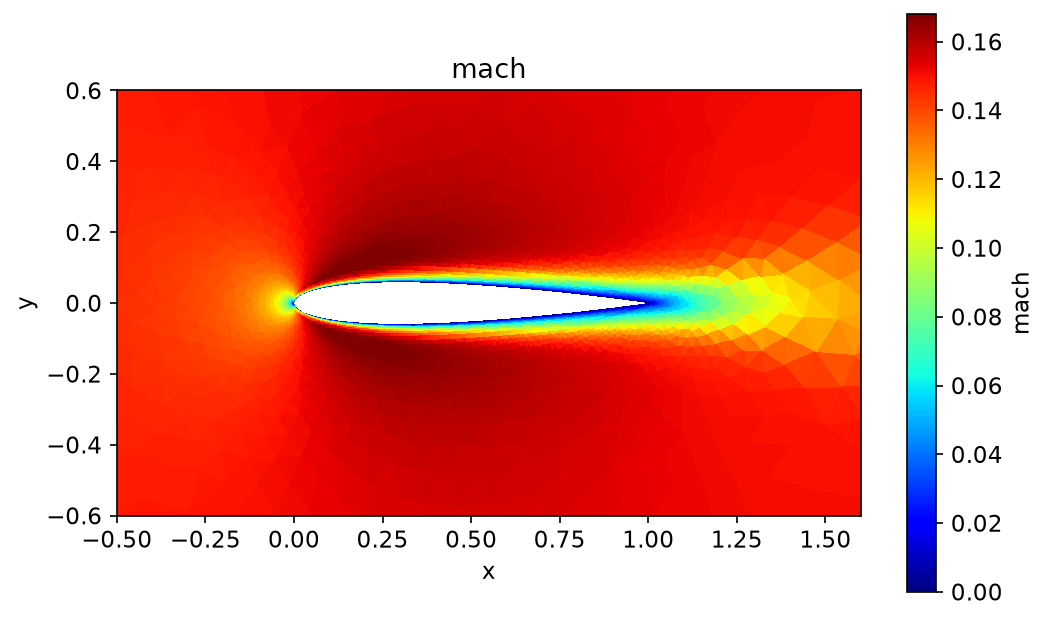
\includegraphics[width=\textwidth]{figures/naca0012_m015_laminar_re5000_mach_zoom.png}
\caption{Mach (near body)}
\end{subfigure}\hfill

\begin{subfigure}{0.48\textwidth}\centering
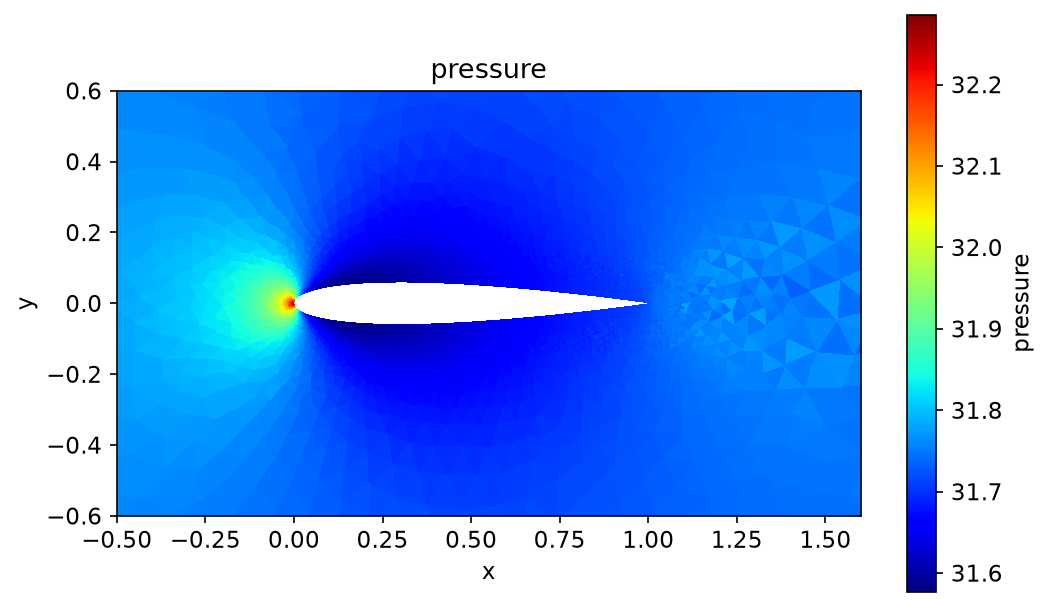
\includegraphics[width=\textwidth]{figures/naca0012_m015_laminar_re5000_pressure_zoom.png}
\caption{pressure (near body)}
\end{subfigure}\hfill
\caption{Case \texttt{naca0012\_m015\_laminar\_re5000}: residual and force histories, surface distributions, and field contours. Plotted variables are named in each subcaption.}
\label{fig:m015lam}
\end{figure}

\begin{figure}[htbp]\centering
\begin{subfigure}{0.48\textwidth}\centering
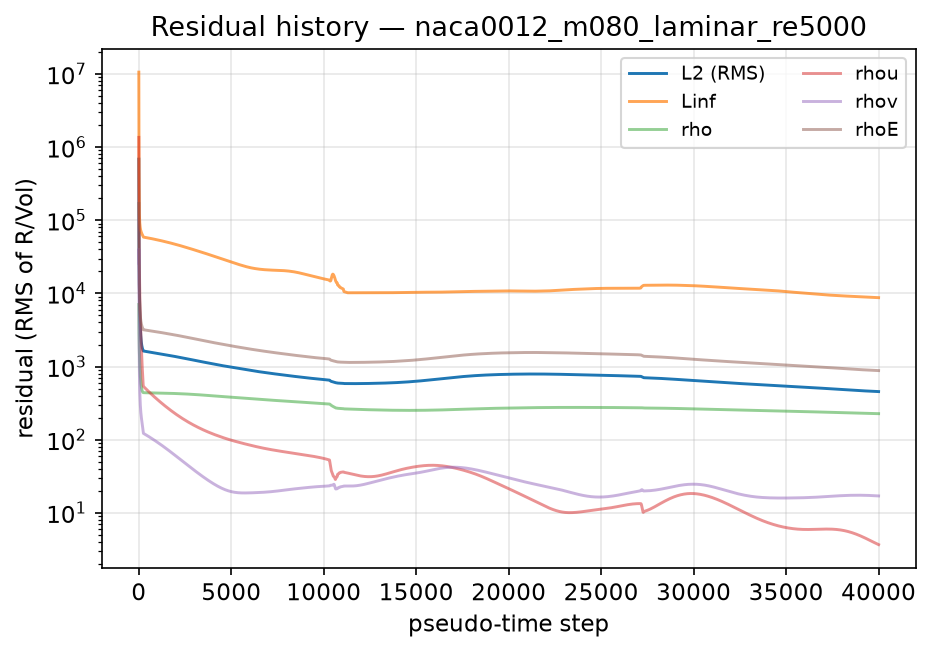
\includegraphics[width=\textwidth]{figures/naca0012_m080_laminar_re5000_residuals.png}
\caption{residual history}
\end{subfigure}\hfill
\begin{subfigure}{0.48\textwidth}\centering
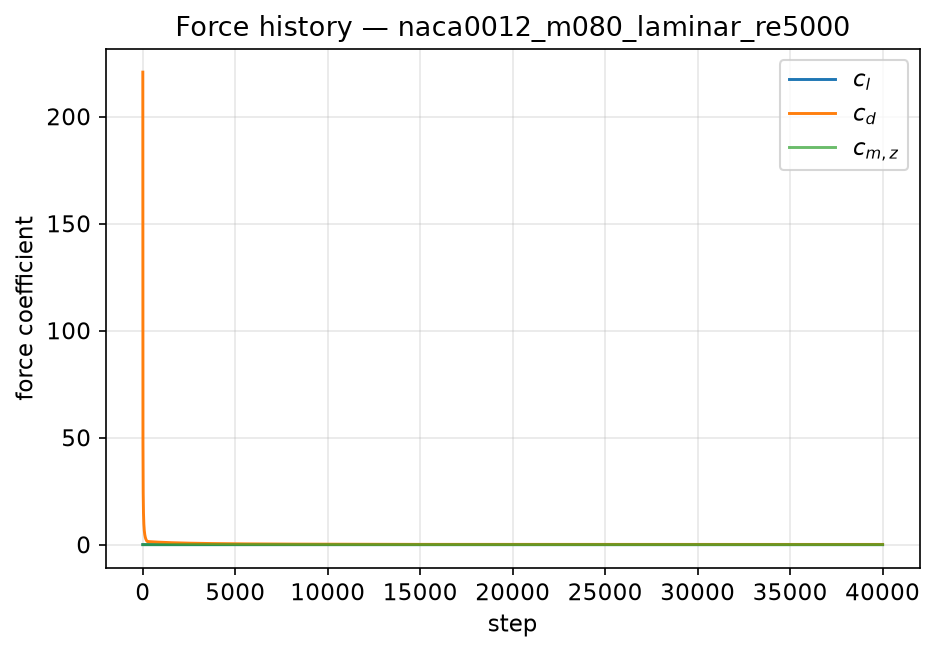
\includegraphics[width=\textwidth]{figures/naca0012_m080_laminar_re5000_forces.png}
\caption{force history}
\end{subfigure}\hfill

\begin{subfigure}{0.48\textwidth}\centering
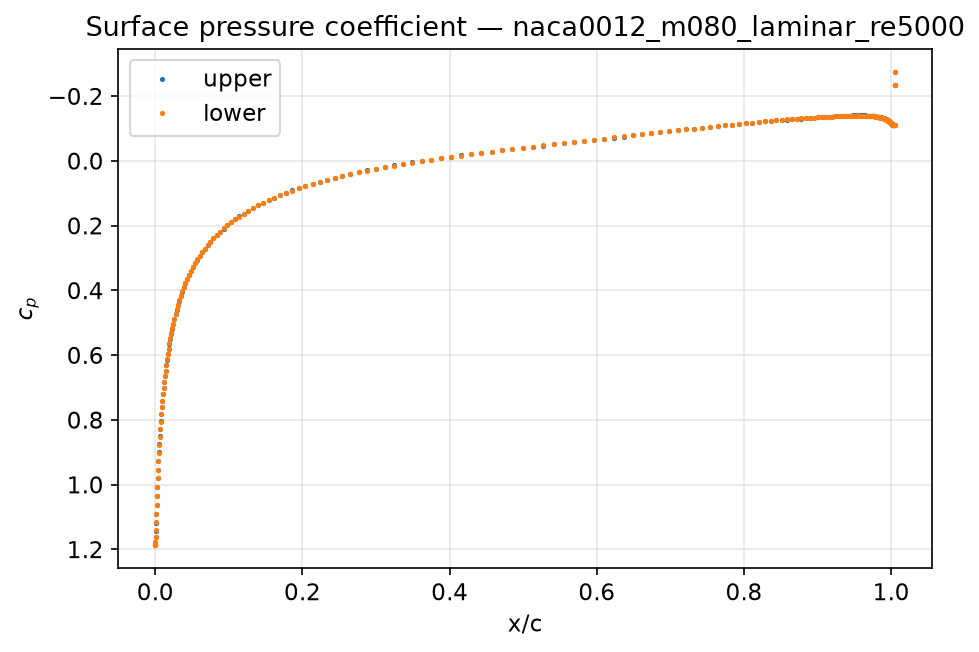
\includegraphics[width=\textwidth]{figures/naca0012_m080_laminar_re5000_surface_cp.png}
\caption{surface $c_p$}
\end{subfigure}\hfill
\begin{subfigure}{0.48\textwidth}\centering
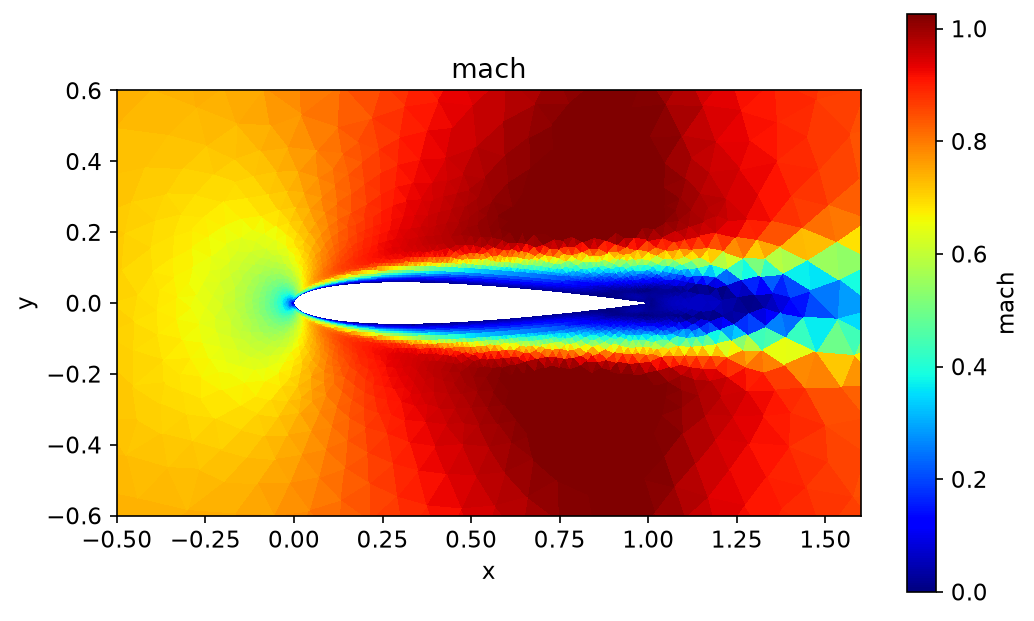
\includegraphics[width=\textwidth]{figures/naca0012_m080_laminar_re5000_mach_zoom.png}
\caption{Mach (near body)}
\end{subfigure}\hfill

\begin{subfigure}{0.48\textwidth}\centering
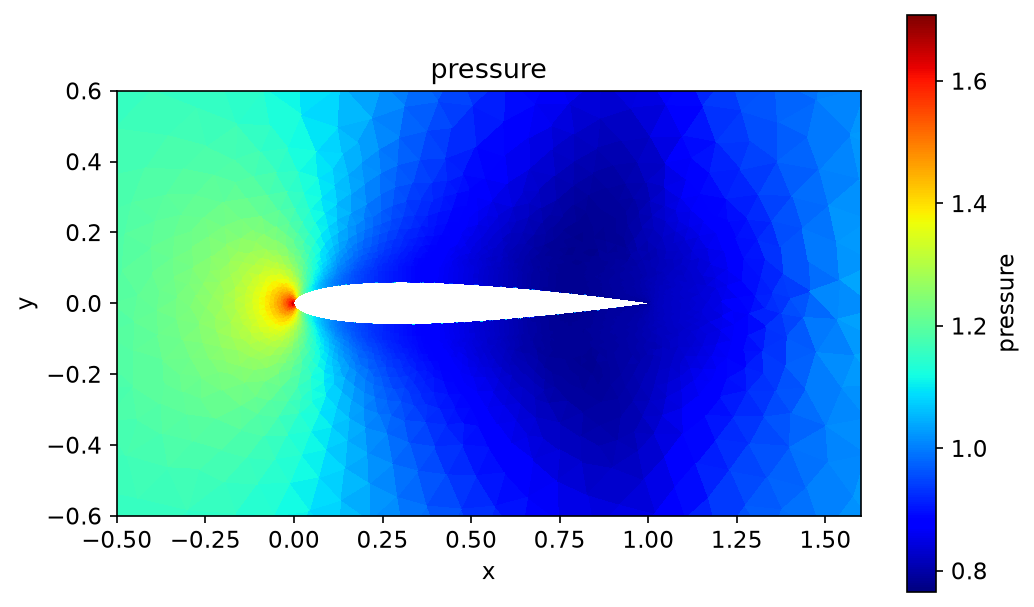
\includegraphics[width=\textwidth]{figures/naca0012_m080_laminar_re5000_pressure_zoom.png}
\caption{pressure (near body)}
\end{subfigure}\hfill
\caption{Case \texttt{naca0012\_m080\_laminar\_re5000}: residual and force histories, surface distributions, and field contours. Plotted variables are named in each subcaption.}
\label{fig:m080lam}
\end{figure}

\begin{figure}[htbp]\centering
\begin{subfigure}{0.48\textwidth}\centering
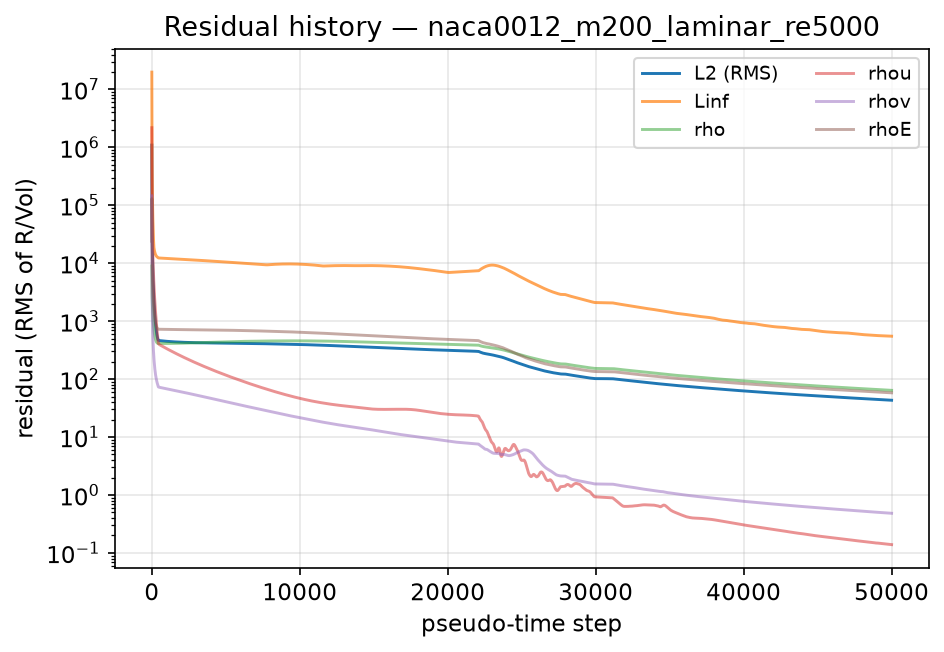
\includegraphics[width=\textwidth]{figures/naca0012_m200_laminar_re5000_residuals.png}
\caption{residual history}
\end{subfigure}\hfill
\begin{subfigure}{0.48\textwidth}\centering
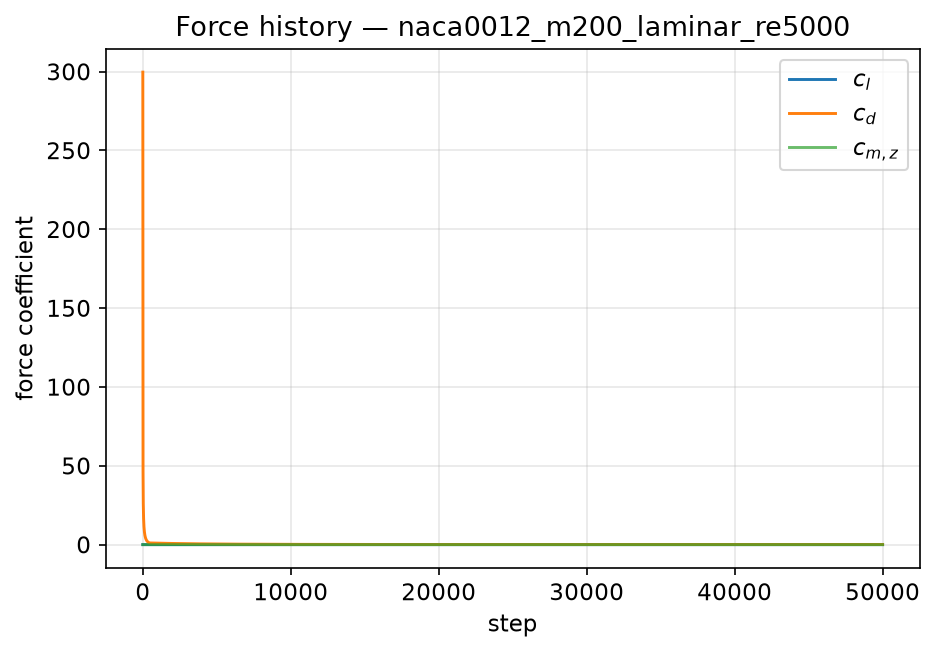
\includegraphics[width=\textwidth]{figures/naca0012_m200_laminar_re5000_forces.png}
\caption{force history}
\end{subfigure}\hfill

\begin{subfigure}{0.48\textwidth}\centering
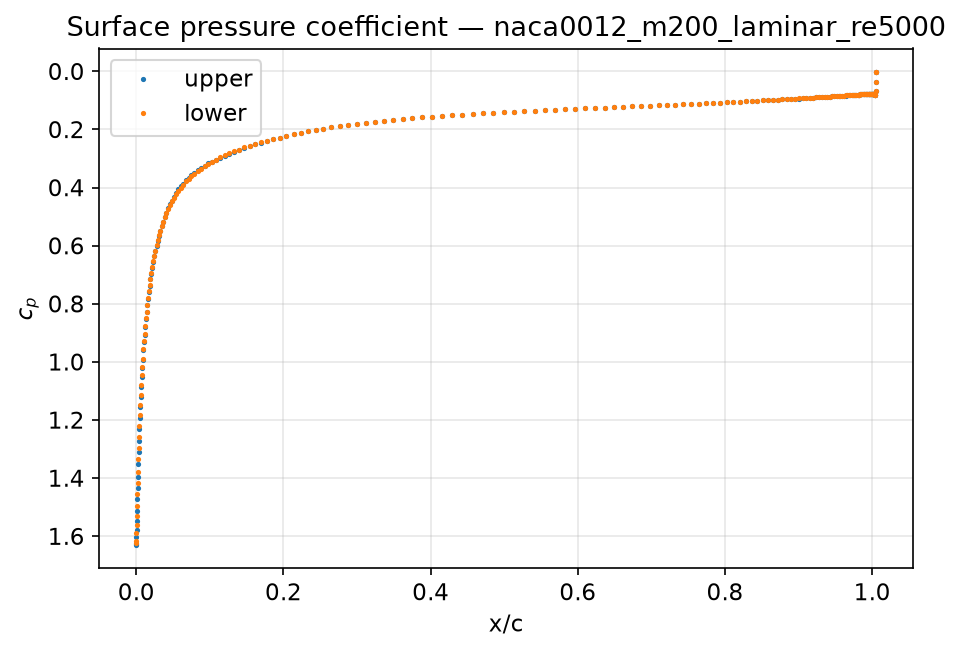
\includegraphics[width=\textwidth]{figures/naca0012_m200_laminar_re5000_surface_cp.png}
\caption{surface $c_p$}
\end{subfigure}\hfill
\begin{subfigure}{0.48\textwidth}\centering
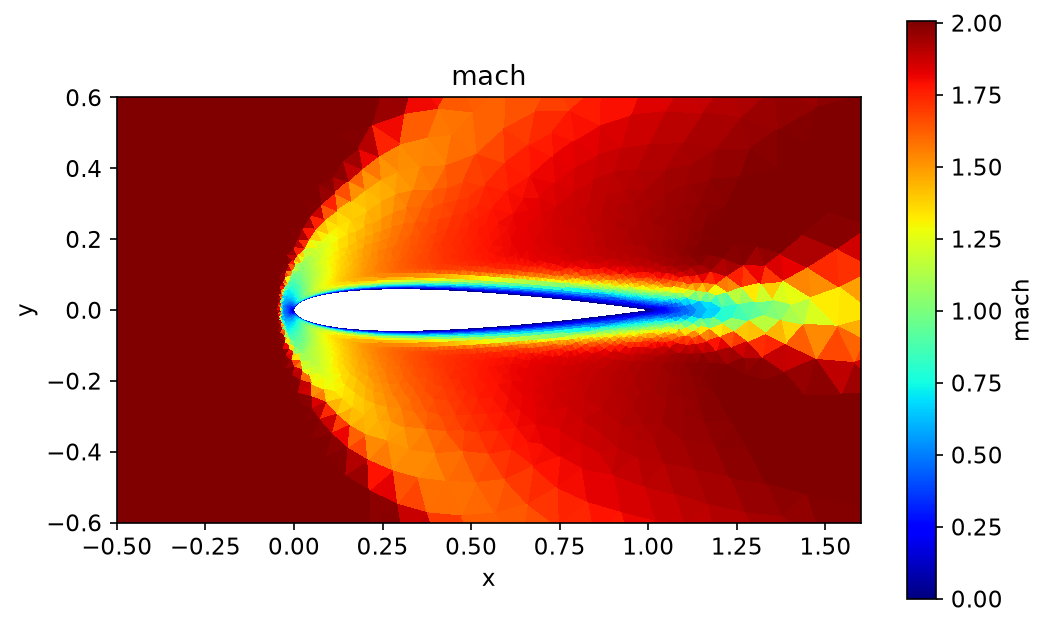
\includegraphics[width=\textwidth]{figures/naca0012_m200_laminar_re5000_mach_zoom.png}
\caption{Mach (near body)}
\end{subfigure}\hfill

\begin{subfigure}{0.48\textwidth}\centering
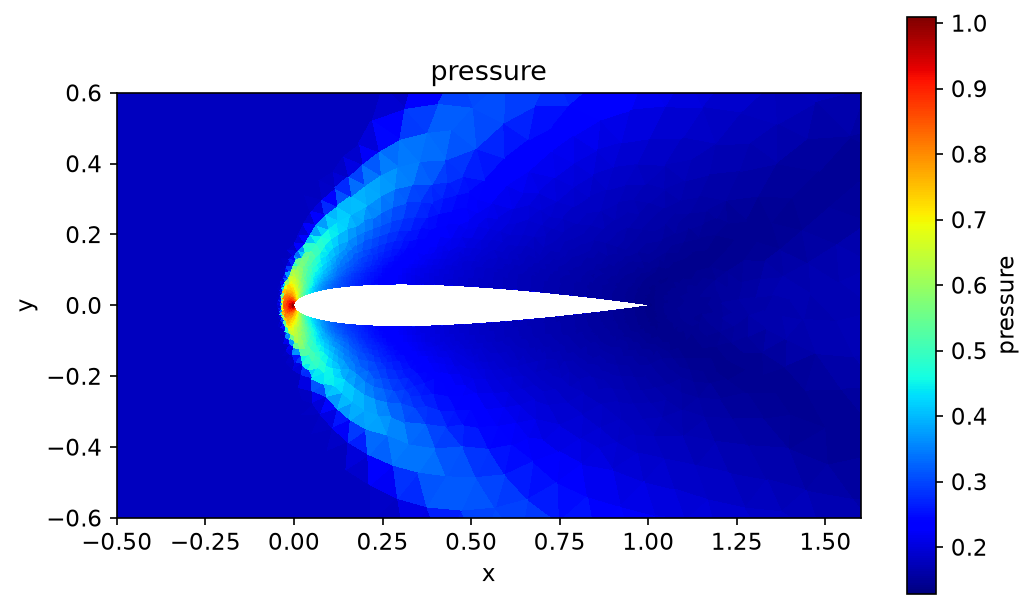
\includegraphics[width=\textwidth]{figures/naca0012_m200_laminar_re5000_pressure_zoom.png}
\caption{pressure (near body)}
\end{subfigure}\hfill
\caption{Case \texttt{naca0012\_m200\_laminar\_re5000}: residual and force histories, surface distributions, and field contours. Plotted variables are named in each subcaption.}
\label{fig:m200lam}
\end{figure}

\begin{figure}[htbp]\centering
\begin{subfigure}{0.48\textwidth}\centering
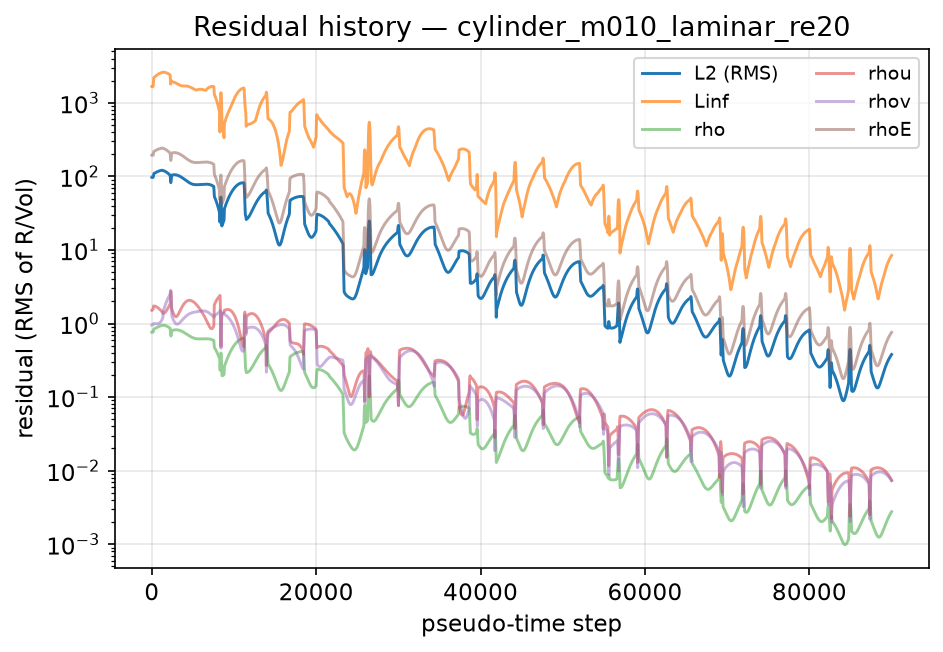
\includegraphics[width=\textwidth]{figures/cylinder_m010_laminar_re20_residuals.png}
\caption{residual history}
\end{subfigure}\hfill
\begin{subfigure}{0.48\textwidth}\centering
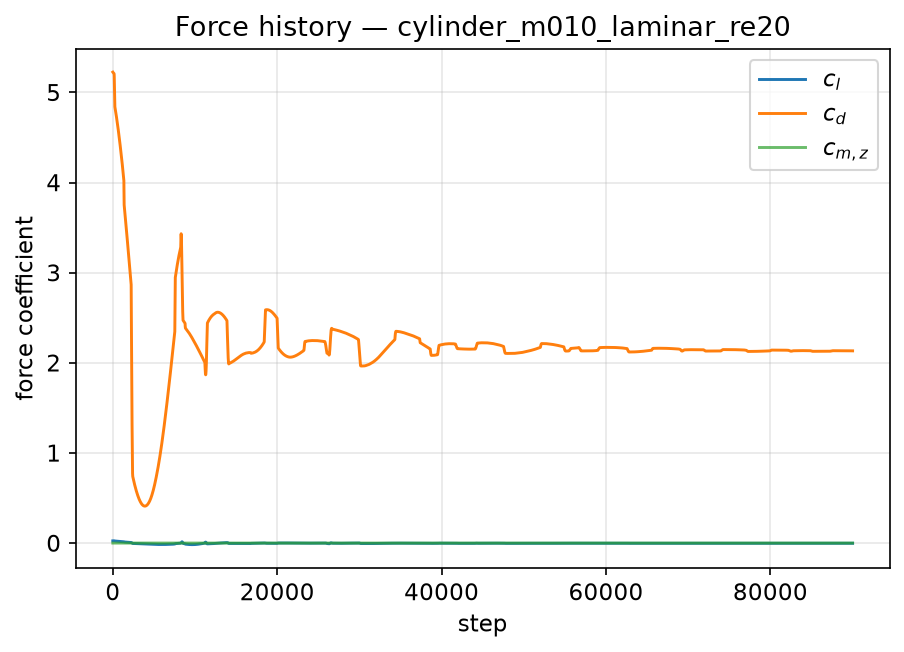
\includegraphics[width=\textwidth]{figures/cylinder_m010_laminar_re20_forces.png}
\caption{force history}
\end{subfigure}\hfill

\begin{subfigure}{0.48\textwidth}\centering
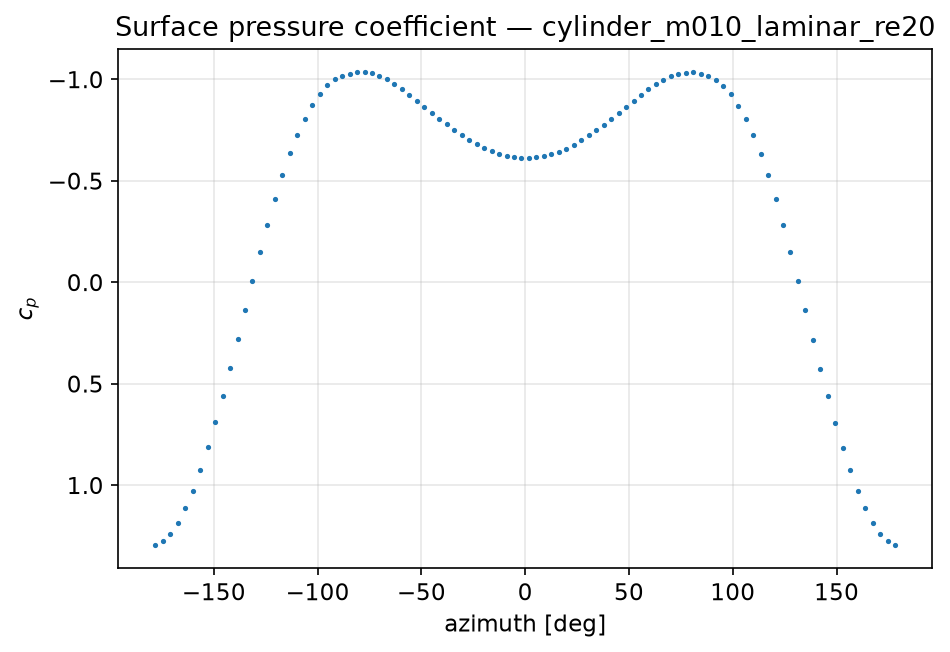
\includegraphics[width=\textwidth]{figures/cylinder_m010_laminar_re20_surface_cp.png}
\caption{surface $c_p$}
\end{subfigure}\hfill
\begin{subfigure}{0.48\textwidth}\centering
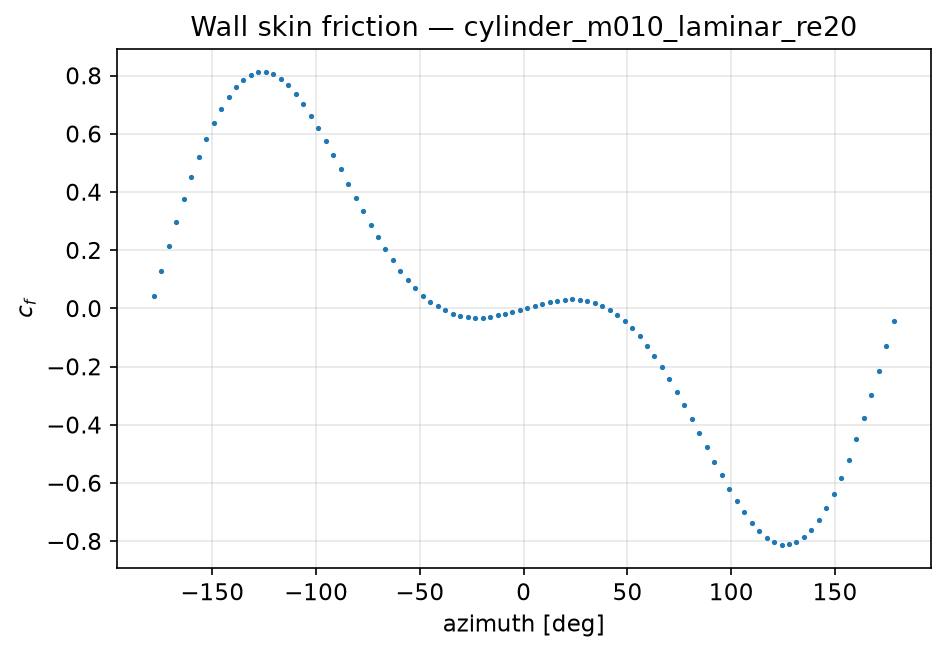
\includegraphics[width=\textwidth]{figures/cylinder_m010_laminar_re20_surface_cf.png}
\caption{surface $c_f$}
\end{subfigure}\hfill

\begin{subfigure}{0.48\textwidth}\centering
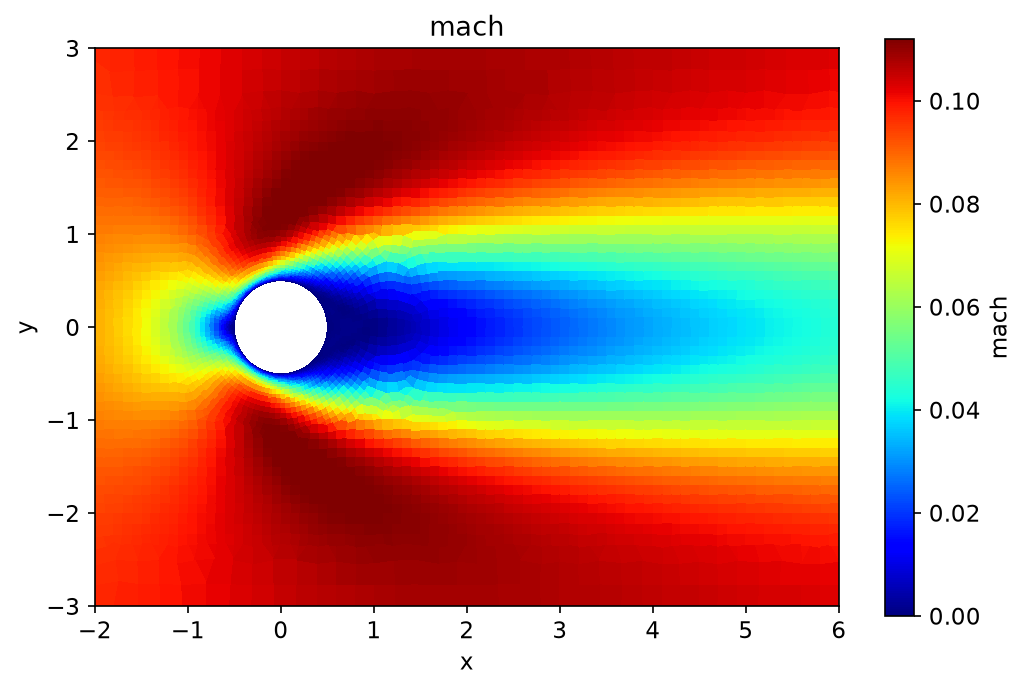
\includegraphics[width=\textwidth]{figures/cylinder_m010_laminar_re20_mach_zoom.png}
\caption{Mach (near body)}
\end{subfigure}\hfill
\begin{subfigure}{0.48\textwidth}\centering
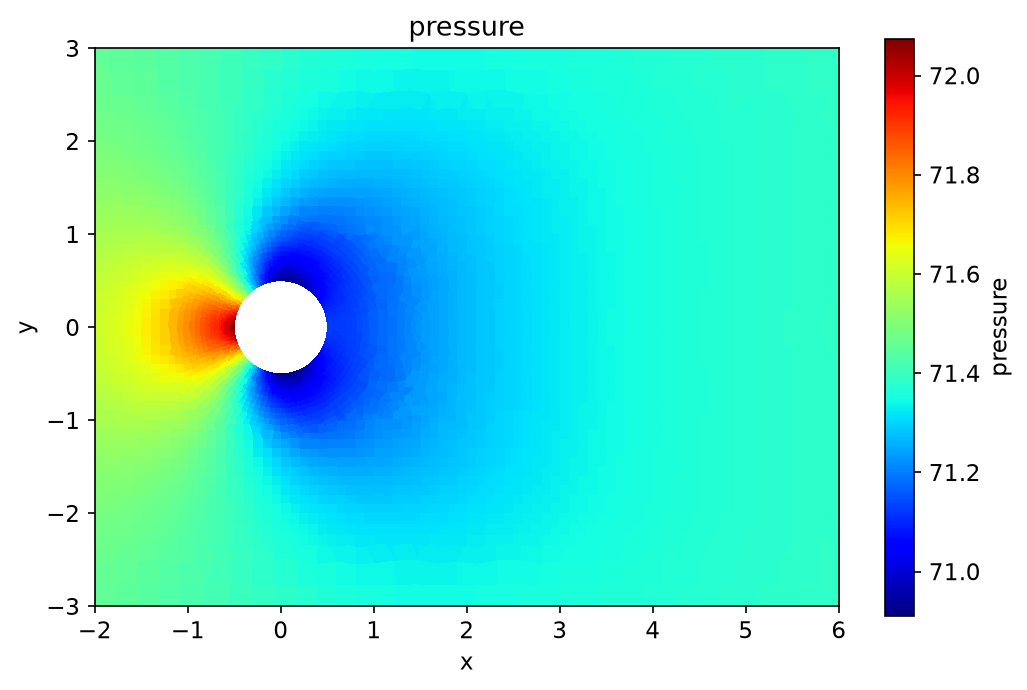
\includegraphics[width=\textwidth]{figures/cylinder_m010_laminar_re20_pressure_zoom.png}
\caption{pressure (near body)}
\end{subfigure}\hfill

\caption{Case \texttt{cylinder\_m010\_laminar\_re20}: residual and force histories, surface distributions, and field contours. Plotted variables are named in each subcaption.}
\label{fig:re20}
\end{figure}

\begin{figure}[htbp]\centering
\begin{subfigure}{0.48\textwidth}\centering
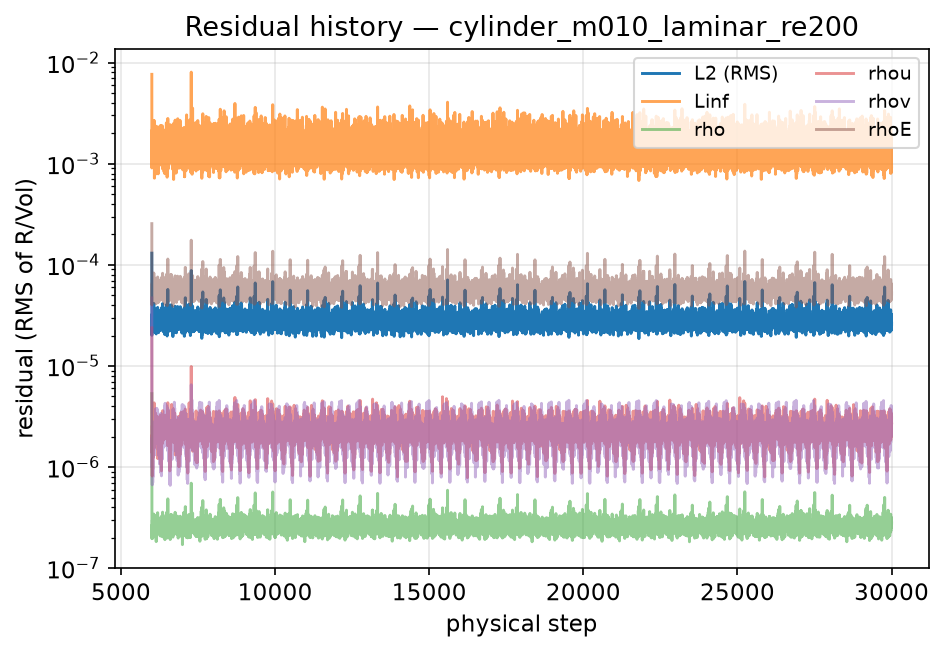
\includegraphics[width=\textwidth]{figures/cylinder_m010_laminar_re200_residuals.png}
\caption{residual history}
\end{subfigure}\hfill
\begin{subfigure}{0.48\textwidth}\centering
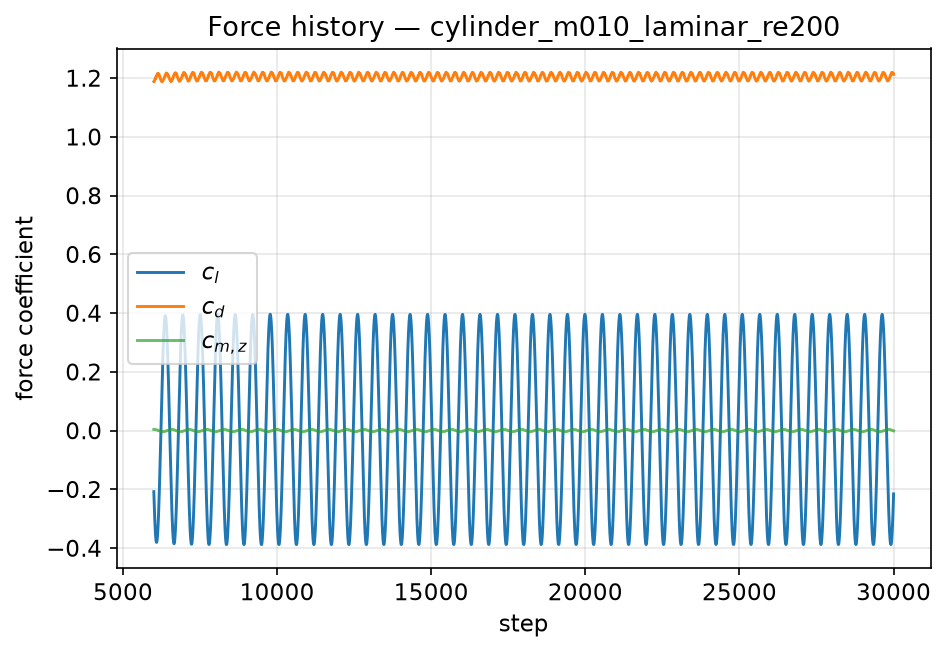
\includegraphics[width=\textwidth]{figures/cylinder_m010_laminar_re200_forces.png}
\caption{force history}
\end{subfigure}\hfill

\begin{subfigure}{0.48\textwidth}\centering
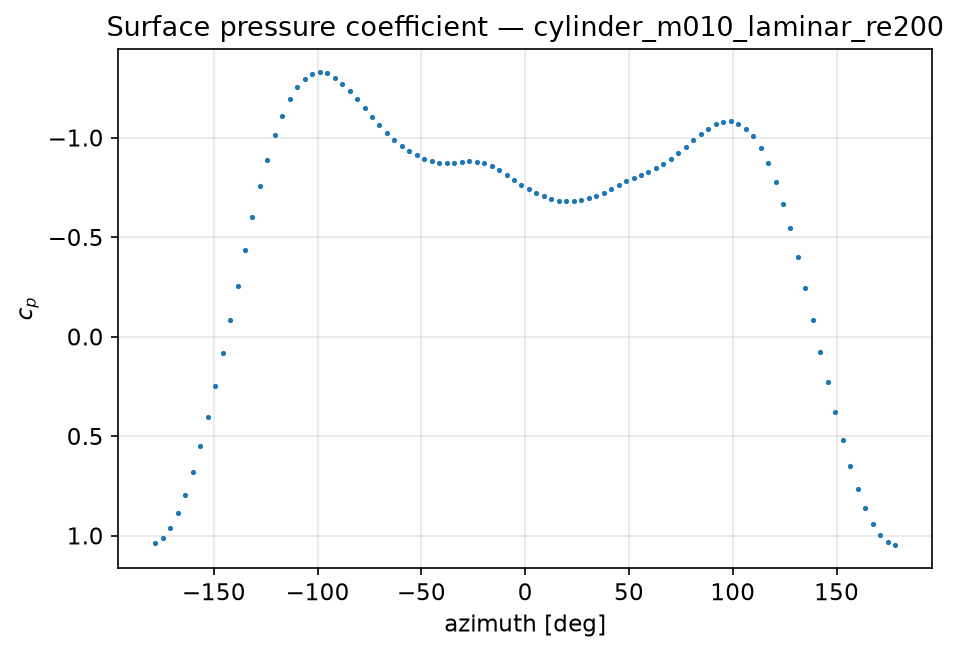
\includegraphics[width=\textwidth]{figures/cylinder_m010_laminar_re200_surface_cp.png}
\caption{surface $c_p$}
\end{subfigure}\hfill
\begin{subfigure}{0.48\textwidth}\centering
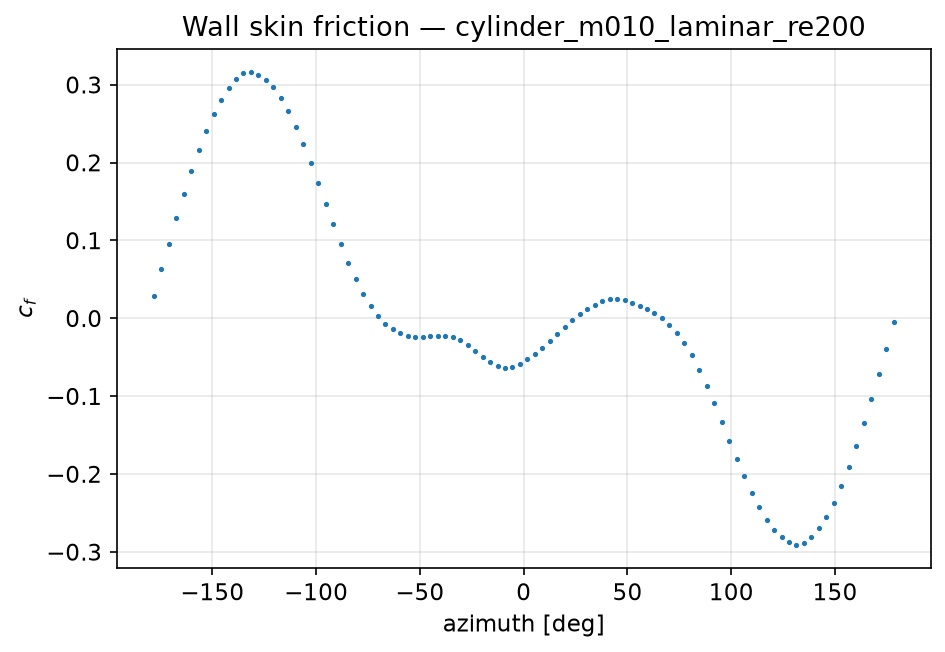
\includegraphics[width=\textwidth]{figures/cylinder_m010_laminar_re200_surface_cf.png}
\caption{surface $c_f$}
\end{subfigure}\hfill

\begin{subfigure}{0.48\textwidth}\centering
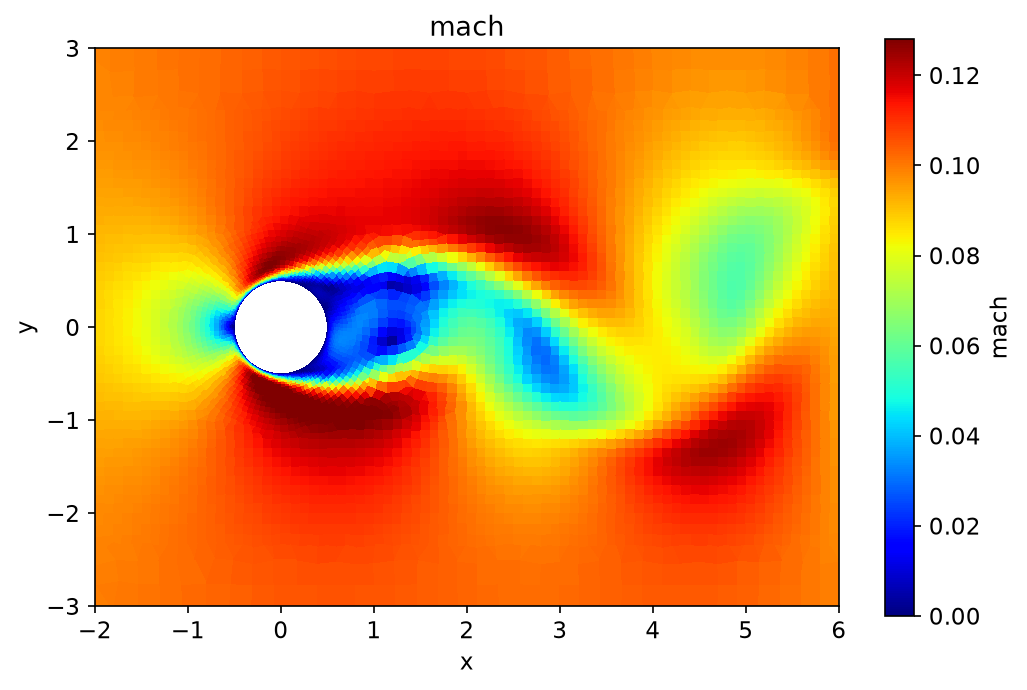
\includegraphics[width=\textwidth]{figures/cylinder_m010_laminar_re200_mach_zoom.png}
\caption{Mach (near body)}
\end{subfigure}\hfill
\begin{subfigure}{0.48\textwidth}\centering
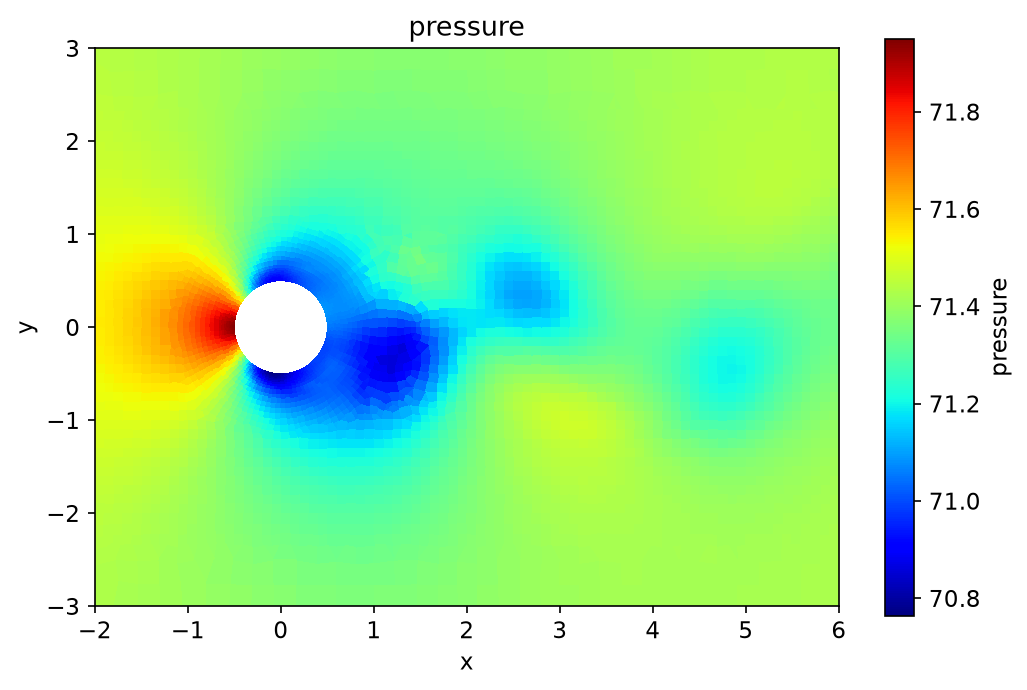
\includegraphics[width=\textwidth]{figures/cylinder_m010_laminar_re200_pressure_zoom.png}
\caption{pressure (near body)}
\end{subfigure}\hfill

\begin{subfigure}{0.48\textwidth}\centering
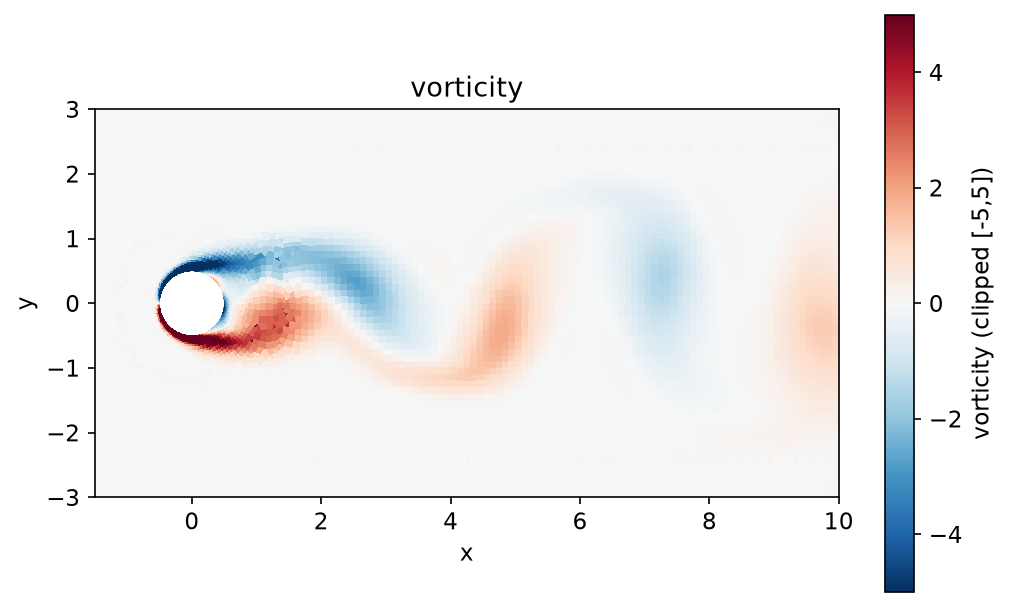
\includegraphics[width=\textwidth]{figures/cylinder_m010_laminar_re200_vorticity_wake.png}
\caption{wake vorticity (clipped)}
\end{subfigure}\hfill
\begin{subfigure}{0.48\textwidth}\centering
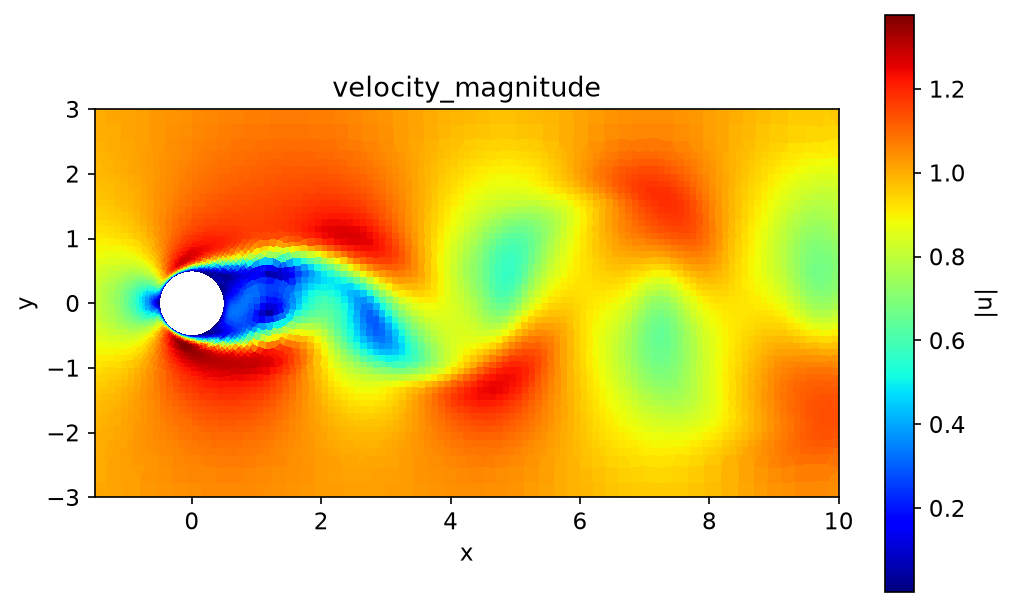
\includegraphics[width=\textwidth]{figures/cylinder_m010_laminar_re200_velocity_wake.png}
\caption{wake velocity magnitude}
\end{subfigure}\hfill

\caption{Case \texttt{cylinder\_m010\_laminar\_re200}: residual and force histories, surface distributions, and field contours. Plotted variables are named in each subcaption.}
\label{fig:re200}
\end{figure}

